\documentclass{article}

\usepackage{amsmath}
\usepackage{fancyhdr}
\usepackage{graphicx}
\graphicspath{{}}

%% some colours
\usepackage{color}
\definecolor{deepblue}{rgb}{0,0,0.5}
\definecolor{deepred}{rgb}{0.6,0,0}
\definecolor{deepgreen}{rgb}{0,0.5,0}
\definecolor{backcolour}{rgb}{0.95,0.96,0.93}

%%%%%%%%%%%%%% CODE STUFF %%%%%%%%%%%%%%
%%%%%%%%%%%%%%%%%%%%%%%%%%%%%%%%%%%%%%%%
\usepackage{cprotect} % to be used in sol
\usepackage{listings} % for code display
% setting code style
\newcommand\pythonstyle{\lstset{
        language=Python,
        backgroundcolor=\color{backcolour},
		basicstyle=\footnotesize,
		otherkeywords={self},
		keywordstyle=\footnotesize\color{deepblue},
		emph={__init__},
		emphstyle=\footnotesize\color{deepred},
		stringstyle=\color{deepgreen},
		frame=single,
		showstringspaces=false  ,
		breaklines=true,
		numbers=left,
		numberstyle=\footnotesize,
		tabsize=4,
		breakatwhitespace=false
	}}

% Python environment
\lstnewenvironment{python}[1][]{
    \pythonstyle
    \lstset{#1}
}{}

% Python for external files
\newcommand\pythonexternal[2][]{{
    \pythonstyle
    \lstinputlisting[#1]{#2}
}}

% Python for inline
\newcommand\pythoninline[1]{{\pythonstyle\lstinline!#1!}}

%%%%%%%%%%%%%%%%%%%%%%%%%%%%%%%%%%%%%%%%
% setting the style for ex documents
\pagestyle{fancy}
\fancyhf{}
\fancyhead[L]{\thetitle}
\fancyhead[C]{}
\fancyhead[R]{\theauthor}
\renewcommand{\headrulewidth}{0.4pt} %obere Trennlinie
\fancyfoot[L]{Due: \thedate}
\fancyfoot[R]{\thepage} %Seitennummer
\renewcommand{\footrulewidth}{0.4pt}

% include solutions
\newcommand\sol[1]{{\large\textbf{\\Solution:}}#1}

\title{BPP Exercise 9 -- Object Oriented Programming}

% {YYYY}{MM}{DD}
\setdate{2019}{06}{09}

\begin{document}


\section{Warm-Up: OOP Quiz (20 points)}

1. Look at the following code snippets. What is the value of {\tt a} and {\tt b} at the end of each of them? Can you explain what the difference is?

\begin{pythoncode}
a = [1, 2, 3]
b = a

# change b
b.append(42)
\end{pythoncode}

\begin{solution}
    The value of {\tt a}, as well as {\tt b} at the end is {\tt [1, 2, 3, 42]}. The reason is, as explained in slides 11-14 in this weeks lecture, that when we write a statement like {\tt a = [1, 2, 3]}, we create a list somewhere, but only store a {\bf pointer} to it in {\tt a}. When we write {\tt b = a}, we just copy the pointer, not the actual object. Now {\tt a} and {\tt b} point to the same object, so if we append to the object in {\tt b}, we also automatically append to the object in {\tt a}.
\end{solution}

\begin{pythoncode}
a = 42
b = a

# change b
b += 10
\end{pythoncode}

\begin{solution}
    In the first two lines, the exact same thing happens. The difference lies in the operations {\tt append} and {\tt +=}. {\tt append} actually {\it mutates} (i.e. changes) the list. {\tt b += 10} can be rewritten as {\tt b = b + 10}, and there you can see the difference: Instead of mutating the object in {\tt b}, we assign a {\it new object} to {\tt b}. This of course does not change the object in {\tt a}.

    \vspace{1em}
\end{solution}

\noindent 2. Decide for each of the statements below whether they are true or false. Give reasons for your answer. When in doubt, base your answer on Python's OOP, not on OOP in other languages.

\begin{enumerate}
    \item An object of {\it class} {\tt Penguin} is also of {\it type} {\tt Penguin}
    \item When an attribute is a {\it property}, it can only be accessed from withtin the object it belongs to
    \item When an attribute starts with an underscore ({\tt \_}), it can only be accessed from within the object it belongs to
    \item {\bf All} of the following things are objects: integers, strings, lists, dictionaries, functions
    \item The constructor is a method that is called when an object is created and is mostly used to define its other methods
\end{enumerate}

\begin{solution}
    \begin{enumerate}
        \item {\bf True.} Well, mostly. In Python, the terms {\it class} and {\it type} are mostly equivalent. We usually talk about user-defined {\it classes} and built-in {\it types}, but this may vary.
        \item {\bf False.} Being a property means to be {\it read-only}, not to be private.
        \item {\bf False} (although true is also an accepted answer if the reasoning is correct). {\tt \_} does signal that an attribute {\it should} not be accessed from outside the object (by convention), but it is still possible.
        \item {\bf True.} In Python, everything you can assign to a variable is an object.
        \item {\bf False.} Yes, the constructor is called on object creation, but it is mostly used to define {\it attributes}, not methods.
    \end{enumerate}
\end{solution}

\section{Modelling with OOP (30 points)}

\subsection{Sketching Ideas}


One Motivation behind Object Oriented Programming is that we can model {\bf real-world entities} with objects. In this assignment, we want to model the entities {\it Human}, {\it Employee} and {\it Student} as {\bf classes}.

\vspace{1em}

\noindent 1. Think of a suitable inheritance structure. Who should inherit from who (i.e. which concept is a specialized version of another concept)? Draw these relationships in a diagram (you can draw on a piece of paper and take a picture if you want). Explain why you chose this structure.

\vspace{1em}

\noindent {\bf Bonus:} Look up the term "UML diagram". It is a standardized way of drawing relationships between classes.

\vspace{1em}

\noindent 2. Think about {\bf attributes} these classes have (at least 3 per class). For example, every human has an age. Keep in mind that attributes get inherited. Write down what attributes you came up with (you can just add them to your diagram, but give a brief explanation if it is not obvious).

\vspace{1em}

\noindent 3. Now think about {\bf methods}. Just with the attributes, define some methods (2 per class) for your classes that make sense. Again, write down your ideas or add them to the diagram.

\vspace{1em}

\begin{solution}
    \begin{center}
        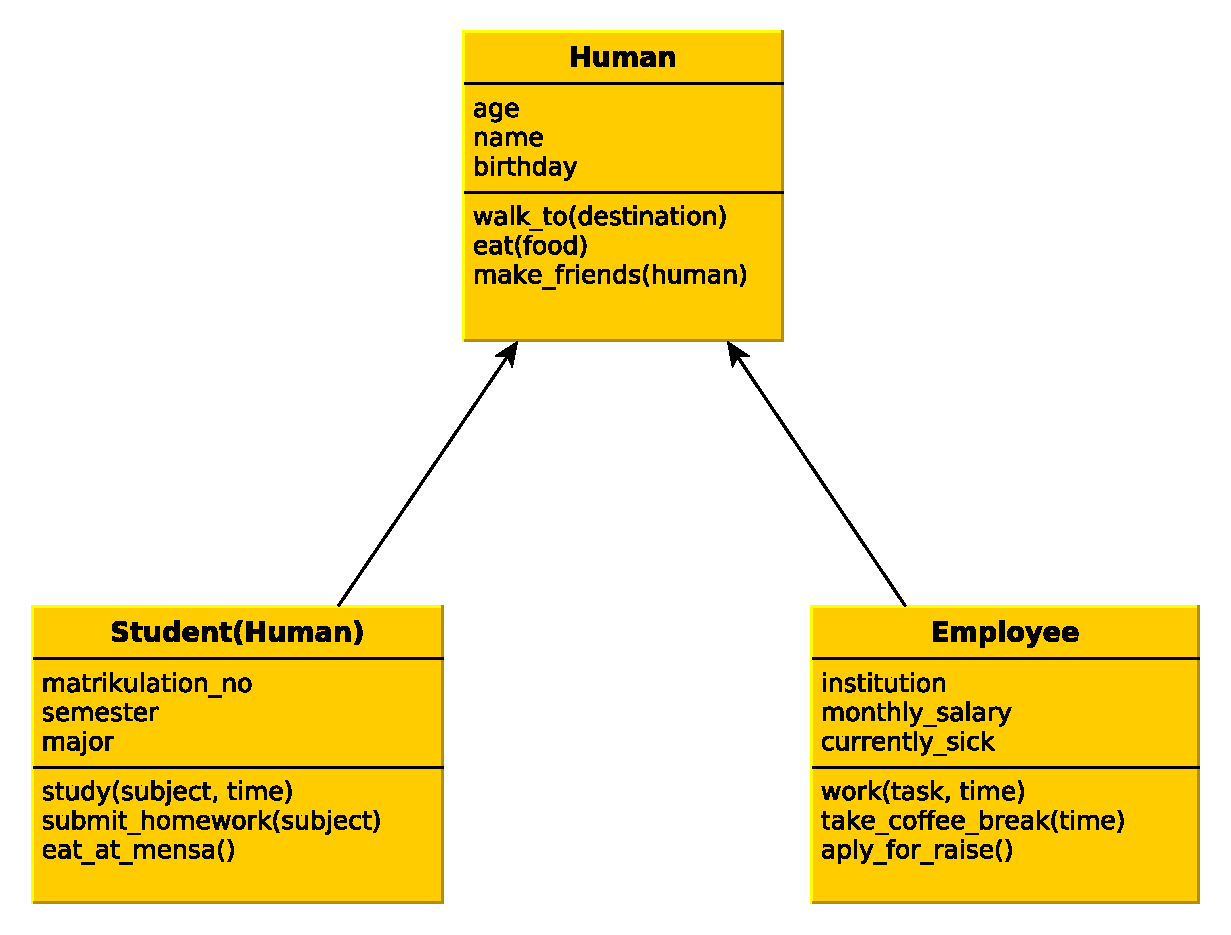
\includegraphics[width=0.5\textwidth]{09_OOP/humans.pdf}
    \end{center}

    \vspace{1em}

    \noindent Both students and employees are humans, so it makes sense for both to inherit from {\tt Human}. They are {\it specialized} concepts of the concept human. Depending on the context, it may or may not make sense for other inheritance relations: perhaps you are modelling student jobs, where every employee is also a student. Then your structure could look like this: {\tt Employee} inherits from {\tt Student}, which inherits from {\tt Human}.
\end{solution}

\subsection{Implementation}

Now it is time to {\it implement} the class structure. Define the three classes you sketched out in 2.1 and give them their methods and attributes. For the methods, it is enough if you leave them empty (e.g. {\tt pass} or {\tt return None}) except for a small docstring that explains what they are supposed to do. Make sure the classes that should inherit from another class do so. Test your implementation by instanciating some objects and checking if they have the methods and attributes that they should have.

\vspace{1em}

\begin{solution}
    \begin{pythoncode}
class Human:
    def __init__(self, name, birthday):
        self.name = name
        self.birthday = birthday

        # this function does not exist, but could be implemented
        self.age = compute_age(current_time(), birthday)

    def walk_to(self, destination):
        pass

    def eat(self, food):
        pass

    def make_friends(self, human):
        pass

class Student(Human):
    def __init__(self, name, birthday, mat_no, semester, major):
        super().__init__(name, birthday)

        self.matrikulation_no = mat_no
        self.semester = semester
        self.major = major

    def study(self, subject, time):
        pass

    def submit_homework(self, subject):
        pass

    def eat_at_mensa(self):
        self.walk_to("mensa")
        self.eat(get_best_mensa_food(today()))

class Employee(Human):
    def __init__(self, name, birthday, institution, salary):
        super().__init__(name, birthday)

        self.institution = institution
        self.monthly_salary = salary
        self.currently_sick = False

    def work(self, task, time):
        pass

    def take_coffee_break(self, time):
        pass

    def apply_for_raise(self):
        pass
    \end{pythoncode}
\end{solution}


\section{Drunk Turtles (30 points)}

Take a look at the file {\tt drunk\_turtles.py}. You will find some code already provided that uses the class {\tt DrunkTurtle}, which inherits from the {\tt Turtle} class of your old friend, the {\tt turtle} module. You should implement this class. The provided code will animate them walking around aimlessly in the empty plains of the turtle world, step by step.

\subsection{The Constructor}

A {\tt DrunkTurtle} cannot walk in a straight line, but walks in random directions. Therefore, the first argument it takes should be an angle that defines how much it can change direction before each step it takes (some turtles are more drunk than others). The second argument it takes should be the size of each step the {\tt DrunkTurtle} takes (some turtles have larger legs than others). The third and last argument is a song the turtle sings while walking around. A song in this context is a {\tt ["list", "of", "words"]}.

\vspace{1em}

\noindent One should be able to construct a {\tt DrunkTurtle} object like this:

\begin{pythoncode}
pete = DrunkTurtle(45, 20, ["Shoo", "wa", "da", "dub."])
\end{pythoncode}

\noindent Because all of these values need to be available by the methods we are going to define later on, you should store them in {\bf attributes}!

\vspace{1em}

\noindent {\bf Bonus - only if you feel like you understand everything so far:} Think of which attributes (and methods from the next step) should be private and how you achieve that in Python.

\subsection{Methods}

Our {\tt DrunkTurtle} will need two methods: {\tt sing} and {\tt move}.

\begin{itemize}
    \item {\tt sing} should take no arguments (besides {\tt self}), and should sing the next word in the song. "sing" in this context means to write the word to the screen at the turtle's current position. You can use the method {\tt write} for that, which {\tt DrunkTurtle} automatically inherits from {\tt Turtle}. You will need to think of a way how {\tt sing} can keep track of where it is in the song.

    \item {\tt move} should also take no arguments. It should rotate the turtle by a random angle from the interval $[-random\_angle, random\_angle]$ and then move it by {\tt step\_size}. The {\tt turtle} functions {\tt forward} and {\tt left} you already know are also available as {\it methods} of {\tt Turtle} objects. It should also call {\tt sing}, because we want to sing one word each step.
\end{itemize}

\subsection{Instances}

Once your class is implemented, fill the two placeholders in the template script with instances of {\tt DrunkTurtle}. Experiment with the arguments and see how they affect the turtles' paths. When you run the script, something like this should unfold:

\begin{center}
    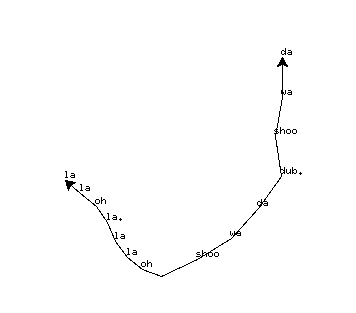
\includegraphics[width=0.5\textwidth]{09_OOP/drunk_turtles.png}
\end{center}

\vspace{1em}

\begin{solution}
    Check the file {\tt drunk\_turtles\_sol.py} for an example solution.
\end{solution}


\section{Thinking Outside the Box: Magic Methods (20 points)}

A {\bf vector} can be described as a collection of numbers, e.g. $(3, 5, 1)$. In two-dimensional vectors (vectors which only have two elements), the first one is often referred to as $x$ and the second as $y$.

\vspace{1em}

\noindent When you {\bf add} two vectors $u$ and $v$, you again get a vector whose elements are the sum of the elements of $u$ and $v$ {\it at the same index}. For example: $(1, 4) + (3, 2) = (1+3, 4+2) = (4, 6)$. This is also called {\it element-wise} addition.

\vspace{1em}

\noindent We would like to use the magic method {\tt \_\_add\_\_} to achieve this behavior in Python. Complete the template of the class {\tt Vector2D} given below.

\begin{enumerate}
    \item First, you need to implement the {\bf constructor}. It is given the $x$ and $y$ values of the vector, which we need to store in attributes.
    \item Next, implement the magic method {\tt \_\_add\_\_}. Besides {\tt self}, it is given the other vector that is supposed to be added to the first one. It should {\it return} their sum, which itself is a {\tt Vector2D}.
    \item Lastly, we want to be able to print a {\tt Vector2D}, just like we can print tuples or lists. For this, the {\tt \_\_str\_\_} method is responsible - it gets called whenever Python tries to convert an object to a string. It should return a string representing the object in some way.
\end{enumerate}

\begin{pythoncode}
class Vector2D:
    def __init__(self, x, y):
        # YOUR CODE HERE

    def __add__(self, other_vector):
        # YOUR CODE HERE

    # ADD DUNDER METHOD __str__ HERE

# testing
u = Vector2D(12, 36)
v = Vector2D(42, 43)

print(u + v)
\end{pythoncode}

\noindent {\bf Intended output (may vary depening on your representation):}

\begin{outputcode}
Vector2D(54, 79)
\end{outputcode}

\begin{solution}
    \begin{pythoncode}
class Vector2D:
    def __init__(self, x, y):
        self.x = x
        self.y = y

    def __add__(self, other_vector):
        """Element-wise addition of two vectors"""
        return Vector2D(self.x + other_vector.x, self.y + other_vector.y)

    def __str__(self):
        """String representation of vector: Vector2D(x, y)"""
        return "Vector2D({}, {})".format(self.x, self.y)
    \end{pythoncode}
\end{solution}

\end{document}
